\clearpage
\refstepcounter{sourcechapter}
\phantomsection
\section*{附录 II\quad 非协调线性有限元的实现}
\label{app:nonconforming-implementation}
\addcontentsline{toc}{section}{附录 II\quad 非协调线性有限元的实现}
\setcounter{section}{-1}
\MBSetSourceChapterAnchor{appendix-02}
\newcounter{appiiproblem}
\renewcommand{\theappiiproblem}{\arabic{appiiproblem}}

\hypertarget{appendix-02-page-336}{}
\begin{center}
\textbf{(逼近 APX5---二维情形)}

F. Thomasset
\end{center}

\section{测试问题}
\label{sec:app2-test-problems}

考虑两个测试问题.

\refstepcounter{appiiproblem}\label{prob:app2-cavity}
\noindent\textbf{问题~\theappiiproblem: 空腔流动.}\quad
$\Omega$ 是平面中的正方形 $(0,1)\times(0,1)$. 在 $\partial\Omega$ 上给定 $u$; 除边 $y=1$ 上 $u=\{U,0\}$ 外, 均有 $u=0$, 其中 $U$ 待指定.

\refstepcounter{appiiproblem}\label{prob:app2-rotating-cylinders}
\noindent\textbf{问题~\theappiiproblem: 非同心旋转圆柱之间的流动.}\quad
$\Omega$ 是平面 $Oxy$ 中由两圆
\[
C_1:x^2+y^2-25=0,
\qquad
C_2:(x-1)^2+y^2-4=0
\]
围成的环形区域. $C_1,C_2$ 分别以待指定的代数角速度 $\sigma_1,\sigma_2$ 旋转.

两种情形均不施加体力.

\section{三角剖分}
\label{sec:app2-triangulation}

三角剖分 $\mathcal T_h$ 由顶点和三角形的编号确定. 自动剖分算法给出如下数组:
\[
X(\cdot),\quad Y(\cdot),
\qquad X(i),Y(i):\text{第 }i\text{ 个顶点的坐标},
\]
\[
Nu(\cdot,\cdot),
\qquad Nu(1,j),Nu(2,j),Nu(3,j):\text{第 }j\text{ 个三角形的顶点编号}.
\]

\hypertarget{appendix-02-page-337}{}
必须能够用简单方式识别边界顶点. 一种经济办法是给它们赋予大于 $N$ 的编号, 其中 $N$ 是内部结点总数.\footnote{若区域有多个边界(即多连通区域), 则还需引入另一组整数, 以区分属于不同边界的点.} 对一般形状区域, 自动剖分算法有两类:\footnote{这里关注一般形状区域的处理. 对需要多次处理的特定几何形状, 当然可能找到比通用程序所得剖分更经济的剖分.}
\begin{itemize}
\item 产生规则网格的``逐次细分''法;
\item Alan George 提出的``区域收缩''法, 适用于具有曲边界的区域.
\end{itemize}

\paragraph{逐次细分法.}
先用粗三角剖分覆盖区域; 此后每一步把每个三角形分成与初始三角形相似的 $k^2$ 个小三角形. 这一过程可重复进行, 直到达到适当的三角形数.

\begin{figure}[htbp]
\centering
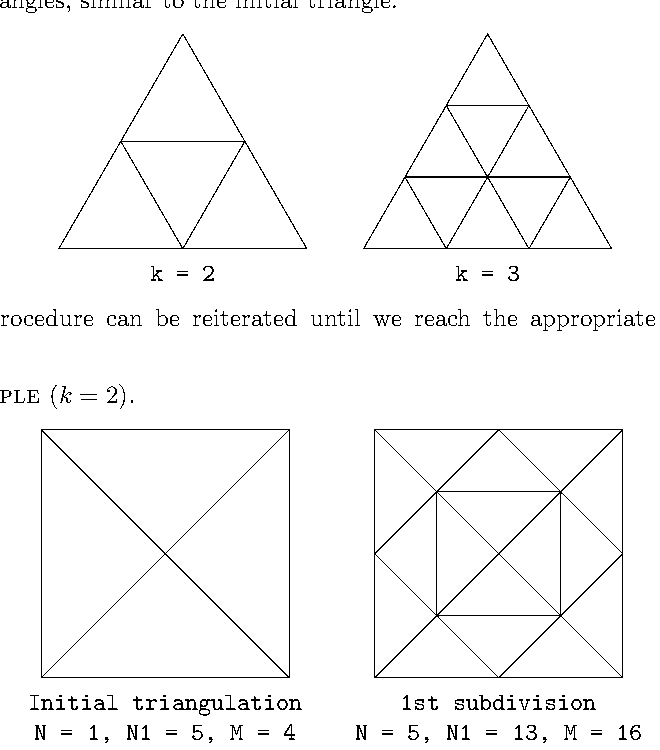
\includegraphics[width=0.58\textwidth]{figures/appendix02-subdivision-diagrams.png}
\caption*{逐次细分示意图}
\end{figure}

例如取 $k=2$. 设给定剖分的内部顶点数、顶点总数和三角形数分别为 $N,N_1,M$. 把每个三角形细分为 $k^2$ 个三角形后, 相应参数记为 $N',N_1',M'$. 注意
\[
2C+C_B=3M,
\qquad C_B=N_1-N,
\]
其中 $C,C_B$ 分别表示内部边数和边界边数, 可得
\[
M'=k^2M,
\]
\[
N'=\frac{(k-1)(k-2)}2M
+\frac{(k-1)(3M+N-N_1)}2+N,
\]
\[
N_1'=N'+k(N_1-N).
\]

\hypertarget{appendix-02-page-338}{}
经过 $n$ 次细分后, 记
\[
M^n=k^{2n}M^0,
\qquad C_B^n=k^nC_B^0,
\]
\[
M^n=2N^n+C_B^n+2(T-1),
\qquad
M^0=2N^0+C_B^0+2(T-1),
\]
其中 $T$ 是区域中孔的数目. 因而三角剖分的参数为
\[
N^n=\frac12\bigl((k^{2n}-1)M^0-(k^n-1)C_B^0\bigr)+N^0,
\]
\[
N_1^n=\frac12\bigl((k^{2n}-1)M^0+(k^n+1)C_B^0\bigr)+N_1^0,
\]
\[
M^n=k^{2n}M^0,
\qquad C_B^0=N_1^0-N^0
\qquad(M^0=M,\ldots).
\]

应当强调, 细分所得三角形与初始剖分的三角形相似, 因而其角不会小于初始剖分中的角. 逐次细分法可适用于具有简单曲边界的区域: 只需把边界边上出现的新顶点替换为它们在 $\partial\Omega$ 上的投影.

\begin{figure}[htbp]
\centering
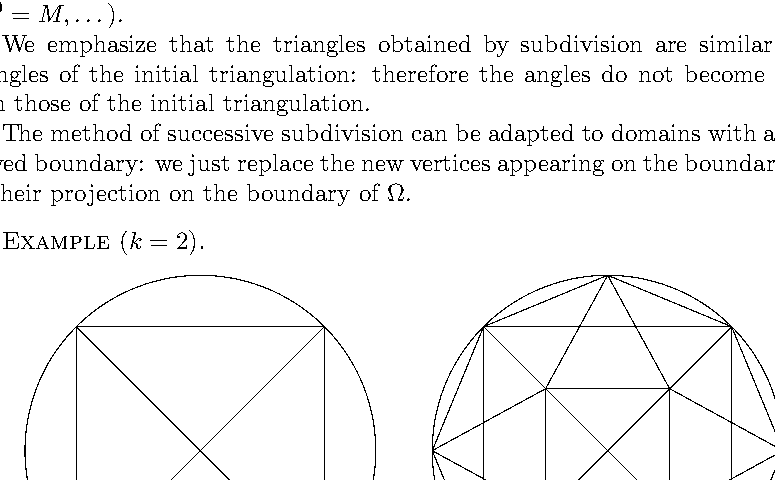
\includegraphics[width=0.62\textwidth]{figures/appendix02-curved-subdivision.png}
\caption*{曲边界区域的逐次细分($k=2$)}
\end{figure}

\paragraph{区域收缩法.}
该方法的原则是用尽可能接近等边三角形的三角形覆盖 $\Omega$; 对等边三角形, 数 $\sigma_T$ 最小, 因而误差界也最小. 先给定 $\partial\Omega$ 的初始离散化, 它由闭合连通的线段序列组成. 若 $\Omega$ 多连通, 必须在 $\Omega$ 中引入人工边界, 剖分完成后再将其删除.

\hypertarget{appendix-02-page-339}{}
给定边界多边形后, 算法可用两种方式构造三角形:
\begin{itemize}
\item 在内部引入新结点(notching);
\item 连接两个相邻边界顶点(trimming).
\end{itemize}
随后从初始区域中去掉最后构造的三角形, 对所得新区域重复上述过程, 直至区域缩减为一个三角形.

\begin{figure}[htbp]
\centering
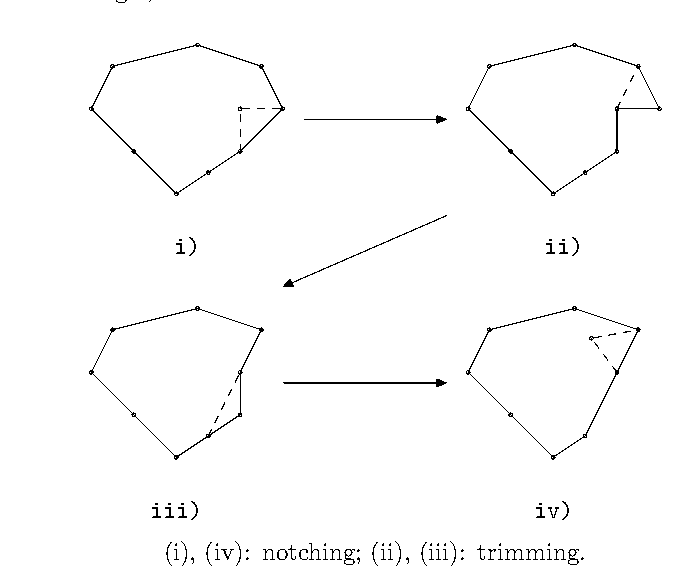
\includegraphics[width=0.56\textwidth]{figures/appendix02-contraction-diagram.png}
\caption*{区域收缩法: (i), (iv)为 notching; (ii), (iii)为 trimming}
\end{figure}

图 \ref{fig:app2-mesh-01}--\ref{fig:app2-mesh-04} 给出两个所考虑几何区域的两种剖分.

\begin{figure}[htbp]
\centering
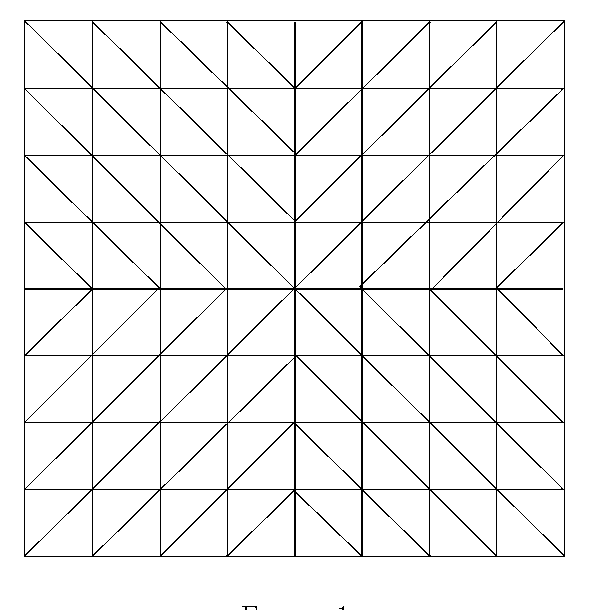
\includegraphics[width=0.46\textwidth]{figures/appendix02-figure01.png}
\caption{}
\label{fig:app2-mesh-01}
\end{figure}

\hypertarget{appendix-02-page-340}{}
\begin{figure}[htbp]
\centering
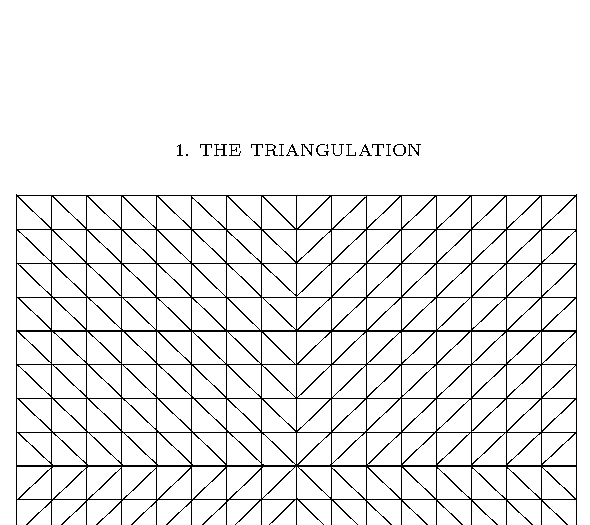
\includegraphics[width=0.46\textwidth]{figures/appendix02-figure02.png}
\caption{}
\label{fig:app2-mesh-02}
\end{figure}

\begin{figure}[htbp]
\centering
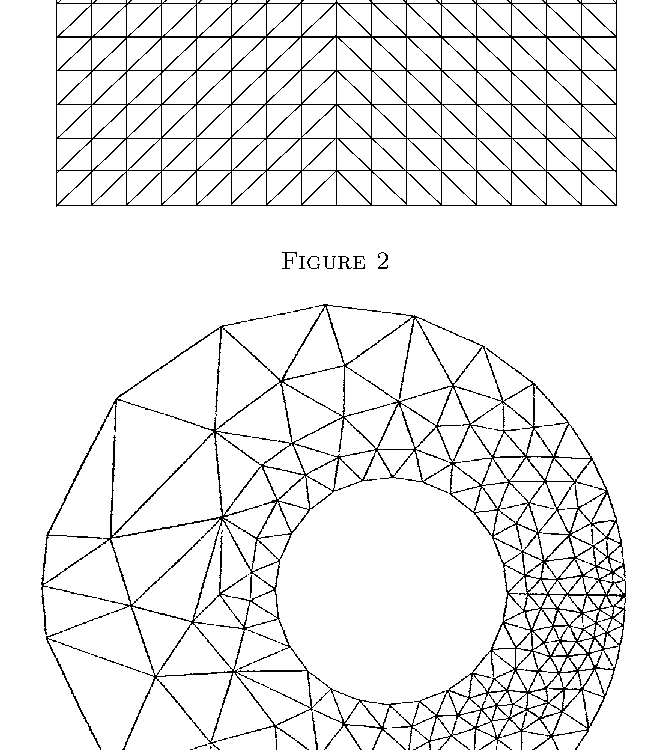
\includegraphics[width=0.54\textwidth]{figures/appendix02-figure03.png}
\caption{}
\label{fig:app2-mesh-03}
\end{figure}

\hypertarget{appendix-02-page-341}{}
\begin{figure}[htbp]
\centering
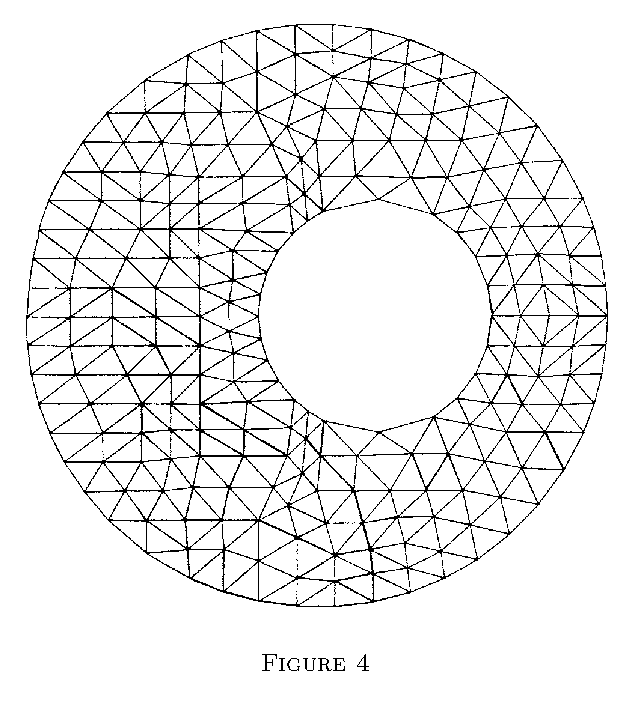
\includegraphics[width=0.52\textwidth]{figures/appendix02-figure04.png}
\caption{}
\label{fig:app2-mesh-04}
\end{figure}

\section{结点}
\label{sec:app2-nodes}

函数 $\phi$ 的结点变量是 $\phi$ 在各边中点处的值, 这些边中点称为结点. 给定数组 $X,Y,Nu$, 构造相应的结点数组
\[
X_m(\cdot),\quad Y_m(\cdot),
\qquad X_m(i),Y_m(i):\text{第 }i\text{ 个结点的坐标}.
\]
边界结点采用大于 $N_m$ 的编号, 其中 $N_m$ 是内部结点数. 再令
\[
Nu_m(\cdot,\cdot),
\qquad Nu_m(1,j),Nu_m(2,j),Nu_m(3,j):\text{第 }j\text{ 个三角形的结点编号}.
\]
这等价于对边进行编号. 后面还需迅速获知给定结点的相邻结点编号, 即与其属于同一三角形的结点; 相邻结点至多有 $4$ 个.

\hypertarget{appendix-02-page-342}{}
\begin{figure}[htbp]
\centering
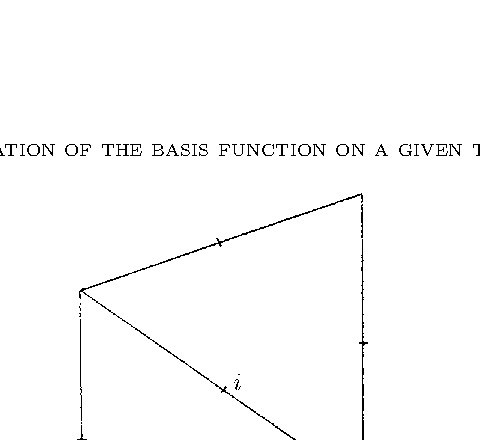
\includegraphics[width=0.34\textwidth]{figures/appendix02-neighbor-diagram.png}
\caption*{一个结点及其相邻结点}
\end{figure}

因此, 由 $Nu_m$ 计算相邻结点数组
\[
TABV(\cdot,\cdot),
\qquad TABV(1,i),TABV(2,i),TABV(3,i),TABV(4,i),
\]
其各项为第 $i$ 个结点的相邻结点编号.

\section{给定三角形上基函数的计算}
\label{sec:app2-local-basis}

给定顶点为 $M_1,M_2,M_3$, 边中点为 $P_1,P_2,P_3$ 的三角形 $T$. 以 $v_1,v_2,v_3$ 表示相应基函数, 即 $v_i(P_j)=\delta_{ij}$. 引入参考三角形 $\widehat T$ 以及把 $\widehat T$ 变换到 $T$ 的线性映射
\[
M=\gamma(\widehat M)
=
\begin{pmatrix}G(1,1)&G(2,1)\\G(1,2)&G(2,2)\end{pmatrix}\widehat M
+\begin{pmatrix}G(3,1)\\G(3,2)\end{pmatrix}.
\]

\begin{figure}[htbp]
\centering
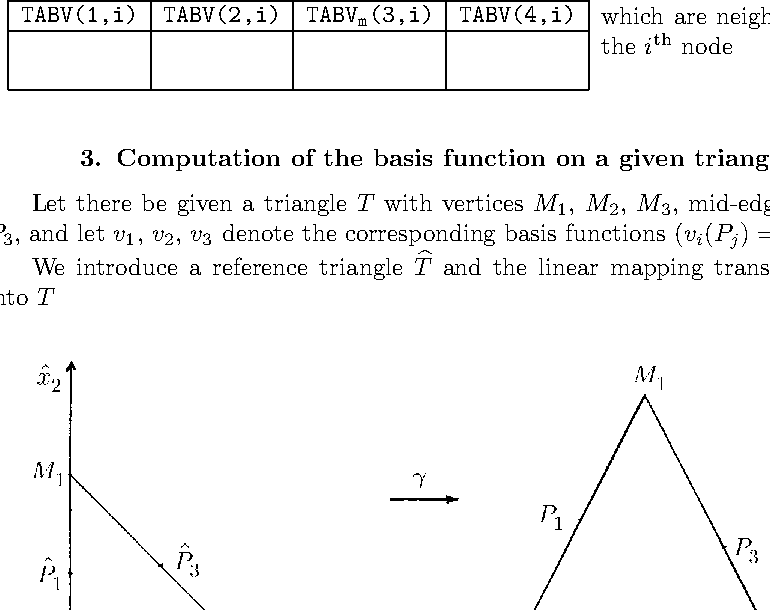
\includegraphics[width=0.58\textwidth]{figures/appendix02-reference-map.png}
\caption*{参考三角形与仿射映射}
\end{figure}

\hypertarget{appendix-02-page-343}{}
利用方程 $M_i=\gamma(\widehat M_i)$ 计算 $G(\alpha,\beta)$:
\[
\begin{aligned}
\begin{pmatrix}G(1,1)&G(2,1)\\G(1,2)&G(2,2)\end{pmatrix}
&=
\begin{pmatrix}(M_1-M_3)_1&(M_2-M_3)_1\\(M_1-M_3)_2&(M_2-M_3)_2\end{pmatrix}
\begin{pmatrix}(\widehat M_1-\widehat M_3)_1&(\widehat M_2-\widehat M_3)_1\\(\widehat M_1-\widehat M_3)_2&(\widehat M_2-\widehat M_3)_2\end{pmatrix}^{-1}\\
&=
\begin{pmatrix}(M_1-M_3)_1&(M_2-M_3)_1\\(M_1-M_3)_2&(M_2-M_3)_2\end{pmatrix}\widehat C,
\end{aligned}
\]
其中 $\widehat C$ 是与 $T$ 无关的 $2\times2$ 矩阵, 且
\[
\begin{pmatrix}G(3,1)\\G(3,2)\end{pmatrix}
=M_1-
\begin{pmatrix}G(1,1)&G(2,1)\\G(1,2)&G(2,2)\end{pmatrix}\widehat M_1.
\]
由 $\gamma$ 容易求得 $\gamma^{-1}$:
\[
\widehat M=\gamma^{-1}(M)
=
\begin{pmatrix}G1(1,1)&G1(2,1)\\G1(1,2)&G1(2,2)\end{pmatrix}M
+\begin{pmatrix}G1(3,1)\\G1(3,2)\end{pmatrix}.
\]

由此具备构造基函数所需的全部信息. 设 $\lambda_i$ 是 $T$ 关于 $M_j$ 的重心坐标, 即 $\lambda_i(M_j)=\delta_{ij}$. 则
\[
v_1=\lambda_1+\lambda_2-\lambda_3,
\quad
v_2=\lambda_2+\lambda_3-\lambda_1,
\quad
v_3=\lambda_3+\lambda_1-\lambda_2.
\]
另一方面, 原书给出
\[
\lambda_1(M)=\widehat x_2(\widehat M),
\quad
\lambda_2(M)=1-\widehat x_1(\widehat M)-\widehat x_2(\widehat M),
\quad
\lambda_3(M)=\widehat x_2(\widehat M),
\]
以及
\[
\int_{\widehat T}\widehat x_1^{i_1}\widehat x_2^{i_2}\,d\widehat x_1d\widehat x_2
=\frac{i_1!i_2!}{(i_1+i_2+2)!}.
\]
由此推出
\[
\operatorname{area}T=\frac12\det G,
\qquad
\int_Tv_1\,dM=\frac13\operatorname{area}(T),
\qquad
\int_Tv_iv_j\,dM=\frac13\delta_{ij}\operatorname{area}(T).
\]
值得注意的是, 基函数在 $L^2(T)$ 中正交. $v_i$ 的梯度可用矩阵 $G1$ 计算:
\[
\frac{\partial\lambda_i}{\partial x_j}
=\sum_{k=1,2}\frac{\partial\widehat x_k}{\partial x_j}
\frac{\partial(\lambda_i\circ\gamma)}{\partial\widehat x_k}
=\sum_{k=1,2}G1(j,k)
\frac{\partial(\lambda_i\circ\gamma)}{\partial\widehat x_k}.
\]

\hypertarget{appendix-02-page-344}{}
换言之,
\[
\frac{\partial\lambda_2}{\partial x_j}=G1(j,2),
\qquad
\frac{\partial\lambda_2}{\partial x_j}=-G1(j,1)-G1(j,2),
\qquad
\frac{\partial\lambda_3}{\partial x_j}=G1(j,1),
\]
以及
\[
\frac{\partial v_1}{\partial x_j}=-2G1(j,1),
\qquad
\frac{\partial v_2}{\partial x_j}=-2G1(j,2),
\qquad
\frac{\partial v_3}{\partial x_j}=2G1(j,1)+2G1(j,2).
\]

右端的数值积分采用
\[
\int_Tf(M)v_i(M)\,dM
\simeq\frac{\operatorname{area}(T)}3f(P_i),
\qquad i=1,2,3.
\]

\section{Stokes 问题的求解}
\label{sec:app2-stokes-solution}

\subsection{基函数}
\label{subsec:app2-stokes-basis}

$W_h$(对 $H_0^1(\Omega)$ 的逼近)的一组基为 $w_i$, $i=1,\ldots,N_m$, 其中:
\begin{itemize}
\item $w_i$ 在每个三角形上线性;
\item $w_i=0$ 在 $\partial\Omega_h$ 上;
\item $w_i$ 在每个结点(即每条边的中点)处为零, 但第 $i$ 个结点除外, 在该处 $w_i(i)=1$.
\end{itemize}
$w_i$ 在三角形 $T$ 上的限制是第 \ref{sec:app2-local-basis} 节定义的三个函数 $v_j$ 之一. $w_i$ 的支集是包含结点 $i$ 的两个三角形之并.

$\mathbf W_h$(对 $H_0^1(\Omega)$ 的逼近)的一组基为
\[
\{(w_i,0),(0,w_i):i=1,\ldots,N_m\},
\]
其中 $N_m$ 是内部结点数. 离散齐次 Stokes 问题给出解
\[
u_h=
\begin{pmatrix}\displaystyle\sum_{i=1}^{N_m}X_iw_i\\[2mm]
\displaystyle\sum_{i=1}^{N_m}Y_iw_i\end{pmatrix},
\]
满足
\[
\nu\sum_{j=1}^{N_m}X_j\alpha_{jk}
=\int_\Omega f_xw_k\,dM
+\sum_T\pi_h(T)\operatorname{area}(T)\frac{\partial w_k}{\partial x}(T),
\]
\[
\nu\sum_{j=1}^{N_m}Y_j\alpha_{jk}
=\int_\Omega f_yw_k\,dM
+\sum_T\pi_h(T)\operatorname{area}(T)\frac{\partial w_k}{\partial y}(T),
\qquad 1\leq k\leq N_m,
\]
并且 $\operatorname{div}(u_h)=0$ 在每个 $T$ 上成立. 系数 $\alpha_{jk}$ 由
\begin{equation}
\alpha_{jk}=\sum_{T(j,k)}\operatorname{area}(T)\nabla w_j(T)\cdot\nabla w_k(T)
\label{eq:app2-stiffness-coefficients}
\end{equation}
计算, 求和遍及与结点 $j,k$ 相邻的全部三角形 $T$.

对非齐次问题, 还引入与边界结点对应的 $w_i$, $i>N_m$. 线性系统保持 \eqref{eq:app2-stiffness-coefficients} 的形式, 但须分别在右端加上
\[
-\sum_{j>N_m}X_j\alpha_{jk},
\qquad
-\sum_{j>N}Y_j\alpha_{jk}.
\]

\hypertarget{appendix-02-page-345}{}
对 $j>N$ 的 $X_j,Y_j$ 已知, 由边界数据给出.

\subsection{Uzawa 算法}
\label{subsec:app2-uzawa}

离散 Uzawa 算法如下. 从任意
\[
\pi_h^0=\{\pi_h^0(T):T\in\mathcal T_h\}
\]
开始, 例如对每个 $T$ 取 $\pi_h^0(T)=0$. 已知 $\pi_h^n$ 后, 计算
\begin{equation}
u_h^{n+1}=
\begin{pmatrix}\displaystyle\sum X_i^{n+1}w_i\\[1mm]
\displaystyle\sum Y_i^{n+1}w_i\end{pmatrix},
\label{eq:app2-uzawa-velocity-expansion}
\end{equation}
其中
\[
\nu\sum_{j=1}^{N_m}X_j^{n+1}\alpha_{jk}
=\int_\Omega f_xw_k\,dM
-\nu\sum_{j>N_m}X_j\alpha_{jk}
+\sum_T\pi_h^n(T)\operatorname{area}(T)\frac{\partial w_k}{\partial x}(T),
\]
\[
\nu\sum_{j=1}^{N_m}Y_j^{n+1}\alpha_{jk}
=\int_\Omega f_yw_k\,dM
-\nu\sum_{j>N_m}Y_j\alpha_{jk}
+\sum_T\pi_h^n(T)\operatorname{area}(T)\frac{\partial w_k}{\partial y}(T).
\]
然后计算
\begin{equation}
\pi_h^{n+1}(T)=\pi_h^n(T)-\rho\operatorname{div}(u_h^{n+1})(T),
\qquad\forall T.
\label{eq:app2-uzawa-pressure-update}
\end{equation}

在 \eqref{eq:app2-uzawa-velocity-expansion} 中, 速度的两个分量实际上是解耦的; 只需求解形如
\begin{equation}
\sum_{j=1}^{N_m}Z_j\alpha_{jk}=f_k,
\qquad k=1,\ldots,N_m,
\label{eq:app2-linear-system}
\end{equation}
的线性系统. 采用超松弛法(S.O.R.)(见 Varga [1]).

\paragraph{超松弛最优参数.}
容易验证矩阵 $(\alpha_{jk})$ 对称正定. 以 $\omega$ 表示松弛参数. 从任意向量 $Z_j^0$ 开始; 已知 $Z_j^n$ 后, 计算
\[
Z_k^{n+1}=(1-\omega)Z_k^n
-\frac{\omega}{\alpha_{kk}}
\left(\sum_{j=1}^{k-1}\alpha_{jk}Z_j^{n+1}
+\sum_{j=k+1}^{N_m}\alpha_{jk}Z_j^n-\frac1\nu f_k\right).
\]
通常采用如下停止判据:
\begin{equation}
\max_k|Z_k^{n+1}-Z_k^n|<\epsilon_{\mathrm{rel}}.
\label{eq:app2-sor-stopping-test}
\end{equation}

松弛参数 $\omega$ 的最优值可由下述算法确定. 对齐次系统
\[
\sum_jZ_j\alpha_{jk}=0
\]
采用 Gauss--Seidel 方法, 初始向量 $Z^0$ 的分量满足 $Z_j^0>0$. 于是
\begin{equation}
Z_k^{n+1}=-\frac1{\alpha_{kk}}
\left(\sum_{j=1}^{k-1}\alpha_{jk}Z_j^{n+1}
+\sum_{j=k+1}^{N_m}\alpha_{jk}Z_j^n\right).
\label{eq:app2-gauss-seidel-iteration}
\end{equation}

\hypertarget{appendix-02-page-346}{}
对每个 $n$ 令
\begin{equation}
\rho_p^{n+1}=\min_k\frac{Z_k^{n+1}}{Z_k^n},
\qquad
\rho_g^{n+1}=\max_k\frac{Z_k^{n+1}}{Z_k^n},
\label{eq:app2-spectral-bounds}
\end{equation}
\begin{equation}
\omega_p^{n+1}=\frac2{1+\sqrt{1-\rho_p^{n+1}}},
\qquad
\omega_g^{n+1}=\frac2{1+\sqrt{1-\rho_g^{n+1}}}.
\label{eq:app2-optimal-relaxation-estimates}
\end{equation}
数值试验表明, $\omega_p^{n+1}$ 和 $\omega_g^{n+1}$ 均收敛到 $\omega_{\mathrm{opt}}$.\footnote{$\rho_p^{n+1}$ 和 $\rho_g^{n+1}$ 收敛到 $\rho(L_1)$, 即 Gauss--Seidel 矩阵的谱半径, 且 $\rho(B)^2=\rho(L_1)$, $\omega_{\mathrm{opt}}=2/(1+\sqrt{1-\rho(B)^2})$.}

\paragraph{矩阵的存储.}
数组 $A$ 存储 $A_0(i)=\alpha_{ii}^0$ 及相邻结点对应的 $\alpha_{i,i_1},\ldots,\alpha_{i,i_4}$; 数组 $TABV$ 存储相邻结点 $i_1,i_2,i_3,i_4$. 若先对结点重新编号, 可用直接法(Cholesky 法、Frontal 法等)求解 \eqref{eq:app2-uzawa-velocity-expansion}; 但在非线性情形使用这些方法并不容易.

\subsection{数值结果}
\label{subsec:app2-stokes-results}

Uzawa 算法中参数 $\rho$ 通过试验选取. 对若干不同的 $\rho$ 进行测试, 并记录给定 Uzawa 迭代次数(例如 $10,20,30,\ldots$)时的结果. 一个良好的收敛性检验量为
\[
C_h^{(n)}=\max_T|\operatorname{div}(u_h^n)_T|.
\]
\footnote{该数等于 $(1/\rho)\max_T|\pi_h^{(n+1)}(T)-\pi_h^n(T)|$, 用于度量离散压力的收敛性. 还考虑 $\delta w_h^{(n)}=\max_i(|X_i^{n+1}-X_i^n|,|Y_i^{n+1}-Y_i^n|)$, 它度量离散速度的收敛性.}

以下给出几何区域 \ref{prob:app2-rotating-cylinders} 的结果, 取 $\nu=1$, $\sigma_1=0$, $\sigma_2=1$; 即 $C_1$ 静止, $C_2$ 以单位角速度旋转, 无体力, 且 $\nu=1$. 图 \ref{fig:app2-uzawa-pressure} 和图 \ref{fig:app2-uzawa-velocity} 清楚显示最优 $\rho$ 的存在; 本例中
\[
\rho_{\mathrm{opt}}=0.96.
\]

\subsection{增广 Lagrange 方法}
\label{subsec:app2-augmented-lagrangian}

这是罚方法与 Uzawa 方法的组合. 在第 1 章 
\MBUnresolvedReference{equation}{(4.209)} 中加入罚项
$(1/\epsilon)(\operatorname{div}_hu_h,\operatorname{div}_hv_h)$, 得到如下方程组(Fortin--Glowinski):
\begin{equation}
\nu((u_h,v_h))_h
+\frac1\epsilon(\operatorname{div}_hu_h,\operatorname{div}_hv_h)
-(\pi_h,\operatorname{div}_hv_h)
=(f,v_h),
\qquad\forall v_h\in\mathbf W_h.
\label{eq:app2-augmented-lagrangian-system}
\end{equation}

\hypertarget{appendix-02-page-347}{}
\begin{figure}[htbp]
\centering
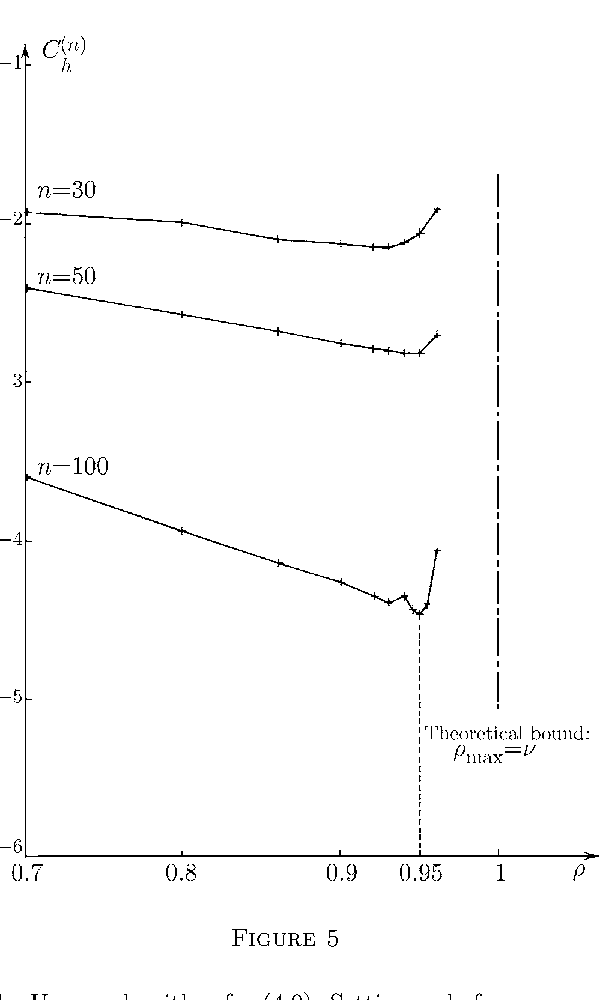
\includegraphics[width=0.48\textwidth]{figures/appendix02-figure05.png}
\caption{}
\label{fig:app2-uzawa-pressure}
\end{figure}

对 \eqref{eq:app2-augmented-lagrangian-system} 写出 Uzawa 算法. 与前面一样令
\[
u_h^{n+1}=\begin{pmatrix}\sum X_i^{(n+1)}w_i\\ \sum Y_i^{(n+1)}w_i\end{pmatrix},
\]
只需把 \eqref{eq:app2-uzawa-velocity-expansion} 的左端替换为
\begin{equation}
\begin{aligned}
&\nu\sum_{j=1}^{N_m}X_j^{n+1}\alpha_{jk}
+\frac1\epsilon\sum_{j=1}^{N_{1m}}
\{X_j^{n+1}(D_{hx}w_j,D_{hx}w_k)
+Y_j^{n+1}(D_{hy}w_j,D_{hx}w_k)\},\\
&\nu\sum_{j=1}^{N_m}Y_j^{n+1}\alpha_{jk}
+\frac1\epsilon\sum_{j=1}^{N_{1m}}
\{X_j^{n+1}(D_{hx}w_j,D_{hy}w_k)
+Y_j^{n+1}(D_{hy}w_j,D_{hy}w_k)\}.
\end{aligned}
\label{eq:app2-augmented-component-system}
\end{equation}
由 \eqref{eq:app2-augmented-component-system} 可见, $X,Y$ 分量的方程不再解耦, 因而要解的线性系统规模是前面研究的 $1/\epsilon=0$ 情形的两倍. 此外, 虽然 S.O.R. 方法可用于求解 \eqref{eq:app2-augmented-component-system}, 但参数 $\omega$ 已不能用第 \ref{subsec:app2-uzawa} 小节的方法求得, 因而只能凭经验选取.

\hypertarget{appendix-02-page-348}{}
\begin{figure}[htbp]
\centering
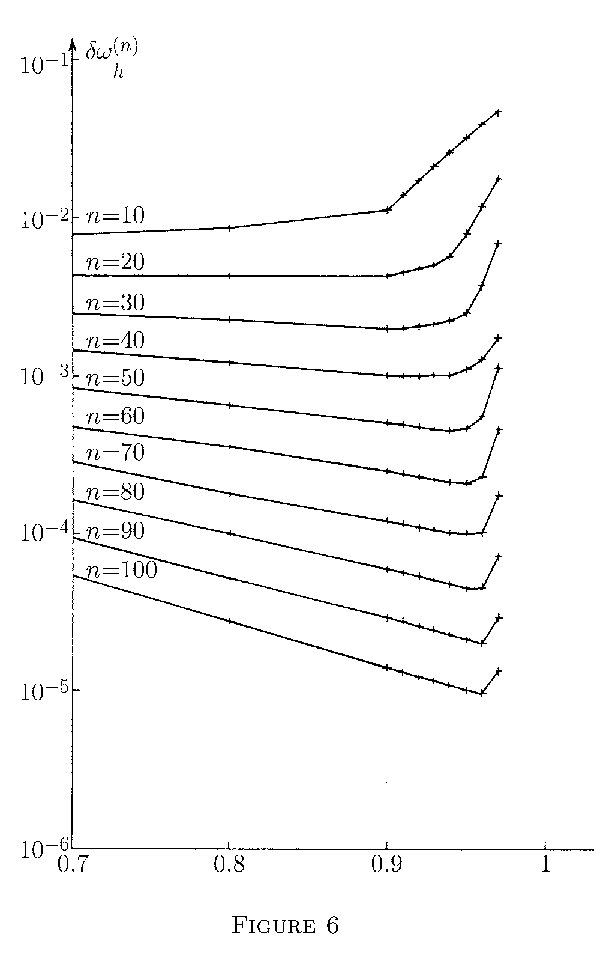
\includegraphics[width=0.48\textwidth]{figures/appendix02-figure06.png}
\caption{}
\label{fig:app2-uzawa-velocity}
\end{figure}

对问题 \ref{prob:app2-rotating-cylinders} 所作试验选取 $\omega=1.6$. 达到收敛($C_h^{(n)}\leq10^{-5}$ 且 $\delta w_h^n\leq10^{-5}$)所需的迭代次数 $n_\epsilon$ 随 $1/\epsilon$ 从零开始增加而减少; 在 $1/\epsilon=8$ 时达到最小, 此时最优 $\rho=\rho(\epsilon)=9.2$. 仅迭代 $15$ 次即达到收敛, 即 $n_\epsilon=15$.

\section{Navier--Stokes 方程的求解}
\label{sec:app2-navier-stokes-solution}

采用如下记号:
\[
\widetilde{\mathbf W}_h:\ H^1(\Omega)\text{ 的逼近},
\qquad
\widetilde W_h:\ H^1(\Omega)\text{ 的逼近},
\]
\[
\mathbf W_h:\ H_0^1(\Omega)\text{ 的逼近},
\qquad
W_h:\ H_0^1(\Omega)\text{ 的逼近}.
\]
$X_h$ 是阶梯函数 $\pi_h$ 的空间; $\pi_h$ 在每个 $S\in\mathcal T_h$ 上为常数, 并在 $\Omega(h)$ 外为零.

\hypertarget{appendix-02-page-349}{}
张成 $W_h$ 的基函数 $v_k$ 对应于 $k\leq N_m$. 令
\[
S_k=\int_{\Omega_h}v_k^2\,dM,
\]
并回顾
\[
\int_{\Omega_h}v_kv_\ell\,dM=0,
\qquad k\neq\ell.
\]
仍引入离散微分算子 $D_{hx}v,D_{hy}v$ 以及离散散度
\[
D_hv=D_{hx}v_x+D_{hy}v_y.
\]
记号 $b_h,a_h$ 与第 2 章 
\MBUnresolvedReference{equation}{(3.78)}, 
\MBUnresolvedReference{equation}{(3.80)} 相同. 离散问题见第 2 章 
\MBUnresolvedReference{equation}{(3.93)}. 我们试验了第 2 章给出的两种算法.

\paragraph{算法 I.}
采用 Uzawa 算法, 见第 2 章 
\MBUnresolvedReference{equation}{(3.107)} 和 
\MBUnresolvedReference{equation}{(3.108)}. 从某个 $p_h^{(0)}\in X_h$ 开始, 例如 $p_h^{(0)}=0$. 已知 $p_h^{(m)}$, $m\geq0$, 后, 计算 $u_h^{m+1}$, 使
\begin{equation}
\nu((u_h^{m+1},v_h))_h
+b_h(u_h^{m+1},u_h^{m+1},v_h)
+\frac1\epsilon(D_hu_h^{m+1},D_hv_h)
=(p_h^m,D_hv_h)+(f,v_h),
\quad\forall v_h\in\mathbf W_h.
\label{eq:app2-navier-stokes-uzawa-velocity}
\end{equation}
方程 \eqref{eq:app2-navier-stokes-uzawa-velocity} 可用欠松弛方法求解. 然后计算
\begin{equation}
p_h^{m+1}=p_h^m-\rho D_hu_h^{m+1}.
\label{eq:app2-navier-stokes-uzawa-pressure}
\end{equation}

\paragraph{算法 II.}
采用隐式 Arrow--Hurwicz 算法, 见第 2 章 
\MBUnresolvedReference{equation}{(3.122)} 和 
\MBUnresolvedReference{equation}{(3.123)}. 按下式计算 $u_h^{m+1}$:
\begin{equation}
\begin{aligned}
&((u_h^{m+1}-u_h^m,v_h))_h
+\rho\left[
\nu((u_h^m,v_h))_h
+\frac1\epsilon(D_hu_h^{m+1},D_hv_h)
+b_h(u_h^m,u_h^{m+1},v_h)\right.\\
&\hspace{42mm}\left.
-(p_h^m,D_hv_h)-(f,v_h)
\right]=0,
\qquad\forall v_h\in\mathbf W_h.
\end{aligned}
\label{eq:app2-arrow-hurwicz-velocity}
\end{equation}
随后由
\[
\alpha(p_h^{m+1}-p_h^m)+\rho D_hu_h^{m+1}=0
\]
定义 $p_h^{m+1}$.

\paragraph{算例.}
图 \ref{fig:app2-cavity-streamlines} 给出问题 \ref{prob:app2-cavity} 在实验所得最佳参数 $\rho,\alpha,\epsilon$ 下的流线: 算法 II, $\nu=10^{-2}$, $U=1$, $512$ 个三角形; 测试了 $1/\epsilon=0,5,7,10$. 图 \ref{fig:app2-cylinder-streamlines} 给出问题 \ref{prob:app2-rotating-cylinders} 的流线: $\nu=4\cdot10^{-2}$, $\sigma_1=1$, $\sigma_2=0$, 采用图 \ref{fig:app2-mesh-04} 的 $412$ 个三角形和 $655$ 个结点; 所选参数为 $\rho=0.1$, $1/\epsilon=10$, $\alpha=0.004$.

\hypertarget{appendix-02-page-350}{}
\begin{figure}[htbp]
\centering
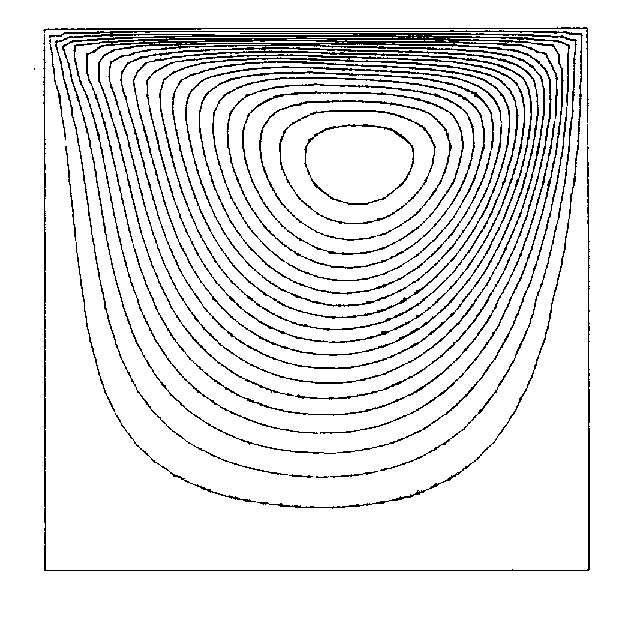
\includegraphics[width=0.48\textwidth]{figures/appendix02-figure07.png}
\caption{}
\label{fig:app2-cavity-streamlines}
\end{figure}

\begin{figure}[htbp]
\centering
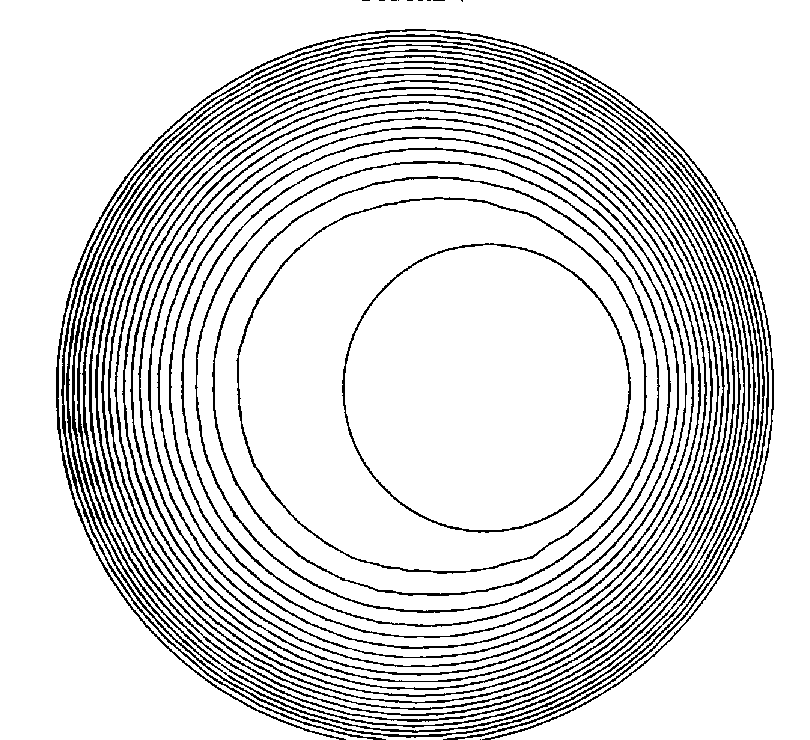
\includegraphics[width=0.60\textwidth]{figures/appendix02-figure08.png}
\caption{}
\label{fig:app2-cylinder-streamlines}
\end{figure}

\hypertarget{appendix-02-page-351}{}
\mbox{}
